\documentclass[12pt,a4paper]{report}

\usepackage[margin=1in]{geometry}
\usepackage{graphicx}
\usepackage{arabtex}
\usepackage{float}
\usepackage{utf8}
\usepackage{caption, subcaption}
\usepackage{hyperref}
\hypersetup{
    colorlinks=false,
    }
\usepackage{cite}
\title{comparative study for machine learning methods used for skin cancer detection and clasification}
\author{
	Khodja Moussa
	\and
	Balbal Oussama
}
\date{}
\begin{document}
\setcode{utf8}

\documentclass[12pt,a4paper]{article}

\usepackage[margin=1in]{geometry}
\usepackage{graphicx}
\title{comparative study for machine learning methods used for skin cancer detection and clasification}
\author{
	Khodja Moussa
	\and
	Balbal Oussama
}
\date{}

\begin{document}
	\begin{titlepage}
		\begin{center}	
			\Large
			
			\includegraphics[]{esi-logo.png}
			
			Ecole Supérieure en Informatique\\
			- 08 Mai 1945- Sidi Bel Abbes
			
			\hrulefill
			
			\vspace{0.5cm}
			\textbf{COMPARATIVE STUDY FOR MACHINE LEARNING METHODS USED FOR SKIN CANCER DETECTION AND CLASSIFICATION}
			%Comparative study for machine learning methods used for skin cancer detection and clasification
			
			\LARGE
			
			\vspace{1.5cm}
			Made by
			\vspace{0.5cm}
			
			\textbf{Khodja Moussa}
			
			\textbf{Balbal Oussama}
			
			\vspace{1.5cm}
			Supervised by
			\vspace{0.5cm}
			
			\textbf{Dr.Meddah Ishak}			
			
			\vfill
			A thesis presented for a master's degree in\\
			\textbf{Computer Systems Engeneering}
			\vspace{0.8cm}
		\end{center}
	\end{titlepage}
\end{document}

\begin{center}
\section*{ACKNOWLEDGEMENT}
\vspace{4cm}
\LARGE
\emph{``We would like to express our special thanks and gratitude to the following people for helping with this master thesis,}\\
\vspace{1cm}
\emph{First of all, We thank Allah the Almighty for giving us courage, and patience needed to complete this work. We would like to thank our parents, families, and friends. We would particularly like to thank our supervisor, Mr. Meddah Ishak, for his competent help, patience and encouragement. May the members of the jury find here the expression of our sincere thanks for the honor they do us by taking the time to read and evaluate this work. We would also like to thank the teaching and administrative team of ESI SBA for their efforts that provided us with excellent training. Finally, I would like to thank everyone who has contributed directly or indirectly to the accomplishment of this work."}
\normalsize
\end{center}
\newpage

\section*{Abstract}
Skin cancer is one of the most common cancers in the world, and it can be fatal if not treated early, that is why its early diagnosis is considered to be the best treatment for it. And under the light of recent advancements in computational power and in the artificial intelligence field (especially its 2 subdomains machine learning and deep learning) C.A.D (computer aided diagnosis) is considered to be one of the best ways for early skin cancer diagnosis. That is why in this article we are going to do a comparative study of recent methods and algorithms applied in skin cancer analysis, detection and classification our comparison is going to be based on different types of datasets used for training, different algorithms applied, and famous performance metrics calculated by researchers such as accuracy, specificity, AUC (area under curve) ...etc. In the hopes of better understanding the problem at hand and its applied solutions, and understanding some new explored ideas and challenges faced by researchers and contributors and finally this article will help new researchers to understand what is ahead of them and get a general view on the various applied methods before engaging and contributing to this field.

\begin{center}
    \RL{الملخص}
\end{center}
\begin{RLtext}

    يعد سرطان الجلد من أكثر أنواع السرطانات شيوعًا في العالم ، ويمكن أن يكون قاتلًا إذا لم يتم علاجه مبكرًا ، ولهذا السبب يعتبر التشخيص المبكر له هو أفضل علاج له. وفي ضوء التطورات الحديثة في القوة الحسابية وفي مجال الذكاء الاصطناعي (خاصةً المجالين الفرعيين للتعلم الآلي والتعلم العميق) ، يُعد \LR{CAD} (التشخيص بمساعدة الكمبيوتر) أحد أفضل الطرق للتشخيص المبكر لسرطان الجلد. هذا هو السبب في أننا سنقوم في هذه المقالة بدراسة مقارنة للأساليب والخوارزميات الحديثة المطبقة في تحليل سرطان الجلد واكتشافه وتصنيفه ، وستستند مقارنتنا إلى أنواع مختلفة من مجموعات البيانات المستخدمة للتدريب ، وخوارزميات مختلفة مطبقة ، و مقاييس الأداء المشهورة التي يحسبها الباحثون مثل الدقة او  (المنطقة تحت المنحنى)  . على أمل فهم المشكلة المطروحة وحلولها التطبيقية بشكل أفضل ، وفهم بعض الأفكار الجديدة المستكشفة والتحديات التي يواجهها الباحثون والمساهمون ، وأخيرًا ستساعد هذه المقالة الباحثين الجدد على فهم ما ينتظرهم قبل الانخراط في هذا المجال والمساهمة فيه. .


\end{RLtext}



\section*{Resumé}
Le cancer de la peau est l'un des cancers les plus répandus dans le monde et il peut être mortel s'il n'est pas traité tôt, c'est pourquoi son diagnostic précoce est considéré comme le meilleur traitement. et à la lumière des avancées récentes en matière de puissance de calcul et dans le domaine de l'intelligence artificielle (en particulier ses 2 sous-domaines d'apprentissage automatique et d'apprentissage profond), la C.A.D (diagnostic assisté par ordinateur) est considérée comme l'un des meilleurs moyens de diagnostic précoce du cancer de la peau. c'est pourquoi, dans cet article, nous allons faire une étude comparative des méthodes et algorithmes récents appliqués à l'analyse, à la détection et à la classification du cancer de la peau. Notre comparaison va être basée sur différents types d'ensembles de données utilisés pour l'entraînement, différents algorithmes appliqués et célèbres indicateurs de performance calculées par les chercheurs telles que la précision, la spécificité, l'AUC (aire sous la courbe) ... etc dans l'espoir de mieux comprendre le problème à résoudre et ses solutions appliquées, et de comprendre certaines nouvelles idées explorées et les défis auxquels sont confrontés les chercheurs et les contributeurs et enfin cet article aidera les nouveaux chercheurs à comprendre ce qui les attend avant de s'engager et de contribuer à ce domaine.

\bigskip
\hrulefill \\
\textbf{Keywords} : Skin cancer - Melanoma - Machine learning - Classification - Diagnostic \\
\vspace{1cm}
\hrulefill \\



\tableofcontents
\listoffigures
\listoftables
\newpage

\chapter{General Introduction}
\section*{General Introduction}
...
% use this article in PFE memoire sent by rahmoun 
% https://medium.com/sliitwif/api-rest-api-and-restful-api-8979bdd64c61?source=email-ed17a7164ab8-1655428466316-digest.reader-de636aa90b4a-8979bdd64c61----0-98------------------86eed88c_c44a_40d5_94d5_f1085845d731-1-

\chapter{General Medecal Information}
\section{Skin}
The skin is a complex organ a ~\cite{elin2018}, it is interactive, self renewing and represents the first and primary defense line against hostile environment and it has several characteristics such as selective absoption, auto regeneration when injured, barrier to water loss, touch sensitivity ...etc ~\cite{joseph2020}. It represents the largest sensory organ (15\% of total body weight and a total area of 1.86 m²) ~\cite{sarah2021}, it has a highly adaptive structure that makes it vital for the survival of the human body, the balance between its static and dynamic properties makes it highly adaptive to the variations of the outer world ~\cite{eliana2022}.

\subsection{Skin Anatomy}
The skin is primary composed of 3 main layers as shown in the figure ~\ref{fig:skin}, each layer has its unique properties and functions ~\cite{sarah2021}.
\begin{description}
\item[Epidermis] the outer most layer which is constantly regenerating and it contains the pigment melanin that determins the skin color and it also represents a physical and biological barrier
\item[Dermis] the middle layer, it supports the flexibility and gives strength the epidermis and it is maily composed of connective tissue
\item[Hypodermis] the last layer which is composed of subcutaneous fat which gives it its properties of being a main support of the overall structure of the skin and shock absoption
\end{description}

%-----------figure skin structure/anatomy ----------------
\begin{figure}[htbp]
\begin{center}
\includegraphics[width=15cm]{./chapter-01-general-medical-information/skin-anatomy.jpg}
\end{center}
\caption{Skin Anatomy ~\cite{fig-skin}}
\label{fig:skin}
\end{figure}

\subsection{Other entities also contained in the skin}
\begin{description}
\item[Hair]  provides protection agains minor trauma, thermoregulation and filtering functions such as nasal hair and eyelashes
\item[Sweat Glands] it is foucd across the entire body, it provides lubrication, temprerature regulation and salt and water balance.
\end{description}
there anatomies are shown in the figure ~\ref{fig:hair}

%-------------figure hair sweat glands-----------------------------
\begin{figure}[htbp]
\begin{center}
\includegraphics[width=15cm]{./chapter-01-general-medical-information/hair-sweat-gland.jpg}
\end{center}
\caption{Hair and Sweat Glands Anatomy ~\cite{fig-hair}}
\label{fig:hair}
\end{figure}


\subsection{Functions of the Skin}
The skin has 6 main functions that can be summarized as follows~\cite{sarah2021}
\begin{description}
\item[Protection]
            the skin is a direct interface between the entarnal organs and the environment so it works as a protective barrier against harmful objects and pathogens (innate/adaptive immunity and unltra-violet light protection  ~\cite{joseph2020}) as shown in figure ~\ref{fig:barrier}
            
\item[Thermostat]
            the skin works as a thermoregulator to keep the body at the optimal temperature of 37 C°, to achieve that is uses multiple strategies such as insensible perspiration, sweating ...etc
\item[Neural relay network]
            the skin contains a dense network of neural endings that works as receptors to various signals and provides sensations for touch, temperature and pain.
\item[Expression and communication]
            A more social function
            is the ability for skin to enable individuals to display
            emotions. It acts as an indicator of one’s physical state.
            Skin is an important component of the stress response as it
            acts as an immediate stress perceiver and as a target of
            stress responses.
            the skin also works as a social tool for interactions between human beings by indicatings the physical state of the individual and by showing sign of stress.
\item[Water storage]
            this skin works as a conservative barrier agains water and body fluids leakage (18-20\% of totla body water) as shown in figure ~\ref{fig:barrier}
\item[Synthesis of vitamin D]
            the skin reperesents the main site of vitamin D production when exposed to the sun, it exists in the plasma membranes of basal and suprabasal keratinocytes in its inactive form then it is converted to previtamin D3 then to Vitamin D in the liver and kidneys  ~\cite{joseph2020} as shown in figure ~\ref{fig:vitaminD}
\end{description}
        %----------figure skin protective barrier-------------
\begin{figure}[htbp]
\begin{center}
\includegraphics[width=15cm]{./chapter-01-general-medical-information/protective-barrier.jpg}
\end{center}
\caption{Protective/moisture Barrier Functions ~\cite{protectiveBarrier}}
\label{fig:barrier}
\end{figure}
        %-----------figure skin vitamin D-----------------
\begin{figure}[htbp]
\begin{center}
\includegraphics[width=10cm]{./chapter-01-general-medical-information/vitaminD.jpg}
\end{center}
\caption{Hair and Sweat Glands Anatomy ~\cite{vitaminD}}
\label{fig:vitaminD}
\end{figure}


\section{Cancer}
        Cancer is an illness caused by the uncontrolled division and spreading of normal cells~\cite{whatiscancer2021} unlike other diseases, cancer is caused by our own bodies and not by foreign entities, and it is one of the biggest causes of death among human beings nowadays (Table ~\ref{tab:cancerStat}) and that is because of the ineffectiveness of traditional treatment methods such as hormones, surgery, radiation, and chemotherapy~\cite{mahsa2022}. Their ineffectiveness is due to their side effects that lead the body to deteriorate more and more. But it is worth mentioning that there are some new methods and approaches being developed by researchers, a couple of those methods are the study of stem cells in relation to cancer cells and the study of the normal cells that the cancer cells came from which are called "Cancer Origin Cells", the latter approach proposes that we should study these origin cells because of their big similarities with cancer cells which will give us a roadmap to its diagnosis and therapy~\cite{rachita2021} .
\begin{table}[htbp]
\begin{center}
\begin{tabular}{|c||c|}
Deaths in 2020 & nealry 10 million \\
\hline
\textbf{Type} & \textbf{New Cases} (millions) in 2020 \\
\hline
Breast &  2.26\\
\hline
Lung &  2.21\\
\hline
Colon and Rectum & 1.93 \\
\hline
Prostate & 1.41 \\
\hline
Skin &  1.20 \\
\hline
Stomach & 1.09 \\
\end{tabular}
\end{center}
\caption{Cancer Statistic ~\cite{cancerStat}}
\label{tab:cancerStat}
\end{table}
\subsection{Origin}
        One of the theories that discuss this is the "carcinogenesis multi-hit theory " which stipulates that for cancer to emerge there are some conditions (hits) that need to be satisfied these hits are produced by genetic mutations (figure ~\ref{fig:mutations}) or rearrangements (figure ~\ref{fig:reaarangement}) that occur over many years and the number of hits necessary is minimal ranging from 3 to 7 only~\cite{rachita2021}. But it is only fair to mention that there are some exceptions to the rule as there are some cancers caused by only one hit. And to go a step further these mutations can be caused by various elements in our environment such as chemicals in tobacco, ultraviolet rays...etc~\cite{whatiscancer2021}.
%----------------------figure mutation-----------------------------
\begin{figure}[htbp]
\begin{center}
\includegraphics[width=15cm]{./chapter-01-general-medical-information/mutation.png}
\end{center}
\caption{DNA Mutation ~\cite{mutations}}
\label{fig:mutations}
\end{figure}
%----------------------figure rearrangements-----------------------------
\begin{figure}[htbp]
\begin{center}
\includegraphics[width=15cm]{./chapter-01-general-medical-information/dna-rearrangement.png}
\end{center}
\caption{DNA Rearrangements ~\cite{reaarangement}}
\label{fig:reaarangement}
\end{figure}
\subsection{Types}
        \subsubsection{According to Fatality}
        \begin{description}
            \item[Benign tumors] \hfill \\
            Are not very harmful because they do not spread to other organs and do not invade nearby tissue, and after removal, they usually don't grow back~\cite{whatiscancer2021} as shown in figure ~\ref{fig:benignMalignant}.
            \item[Malignant tumors] \hfill \\
            Fatal if not treated, because they travel to distant places and form other tumors and invade nearby tissue~\cite{whatiscancer2021} which makes it very hard to remove all its parts, as shown in figure ~\ref{fig:benignMalignant}.
%-----------benign malignant------------------------
\begin{figure}[htbp]
\begin{center}
\includegraphics[width=15cm]{./chapter-01-general-medical-information/benign-malignant.png}
\end{center}
\caption{Benign and Malignant tumors  ~\cite{benignMalignant}}
\label{fig:benignMalignant}
\end{figure}
        \end{description}
            \subsubsection{According to Origin}
            Cancer is also categorized according to where it originated or its origin cells, in this category, there are over 100 types because of the different places it can appear (lung cancer, brain cancer ...)and the different origin cells that it can come from~\cite{whatiscancer2021}.
            \begin{description}
                \item[Carcinoma] \hfill \\
                Most common type formed by epithelial cells.
                \item[Sarcoma] \hfill \\
                Form in bone and soft tissue.
                \item[Leukemia] \hfill \\
                Form in bone marrow, this type does form a tumor but travels in the blood.
                \item[Melanoma] \hfill \\
                Formed by melanocytes (cells that make melanin that gives the skin its color)
                ...etc.
            \end{description}

\section{Skin Cancer}

        Skin cancer is the abnormal growth of cells found in the epidermis (the outer layer of the skin)~\cite{scf2022}, it is one of the most common cancers in the world ~\cite{nhs2020} and it falls under the category of a malignant tumor that is formed by fast multiplication of cells wich is caused by mutations/damage in the DNA  of those cells, the damage in there DNA is due to the exposure to ultra violet rays ~\cite{scf2022} which can come from various sources but the most common are sun light and tanning beds [figure tannig bed] ~\cite{mayo2020, scf2022, nhs2020}. The most common types of skin cancer are  basal cell carcinoma, squamous cell carcinoma , melanoma. The good news is that if it is descovered in an early stage or pre cancurous stage it can be treated easily without leaving a scar.

    %--------tannig bed and sunlamps---------


\subsection{Symptoms} 
        Skin cancer can appear in any place on the body that is exposed to sunlight like : face, scalp, chest ...etc, but there are some cases where the cancer appeared in areas not always exposed to sunlight such as  palm, soles, under the finger neils ~\cite{mayo2020}.
        Skin cancer can happen to people of any skin color but it is know that people with darcker skins are less likely to have it because of the protection against ultra violet rays provided by the melanin which present in darcker people in more quantities than pale people ~\cite{mayo2020}.

        \begin{enumerate}
        \item Basal cell carcinoma signs and symptoms Figure ~\ref{fig:basal}
            \begin{itemize}
            \item bump
            \item flat brown scar
            \item bleeding sore that heals and returns
            \end{itemize}
        \item Squamous cell carcinoma signs and symptoms Figure ~\ref{fig:squamous}
            \begin{itemize}
            \item red nodule
            \item flat lesion with crusted surface
            \end{itemize}
        \item Melanoma signs and symptoms Figure ~\ref{fig:melanoma}
            \begin{itemize}
            \item brownish spot
            \item painful lesion that itches and burns
            \item dark lesion
            \end{itemize}
        
        \end{enumerate}
        
        %------figure of the three---------
        \begin{figure}[h]
        \centering
            \begin{subfigure}[b]{0.3\textwidth}
                \centering
                \includegraphics[scale=.5]{./chapter-01-general-medical-information/Melanoma.jpg}
                \caption{Melanoma ~\cite{wiki2022}}
                \label{fig:melanoma}
            \end{subfigure}
            \begin{subfigure}[b]{0.3\textwidth}
                \centering
                \includegraphics[scale=.3]{./chapter-01-general-medical-information/Squamous.png}
                \caption{Squamous ~\cite{wd}}
                \label{fig:squamous}
            \end{subfigure}
            \begin{subfigure}[b]{0.3\textwidth}
                \centering
                \includegraphics[scale=.5]{./chapter-01-general-medical-information/basal.jpeg}
                \caption{Basal ~\cite{epr2021}}
                \label{fig:basal}
            \end{subfigure}
        \caption{3 Most Common Types of Skin Cancer}
        \label{fig:3types}
        \end{figure}


    \subsection{Types}
        The 3 most common types are the following ~\cite{scf2022}
        \begin{description}
        \item[Basal cell carcinoma] \hfill \\
            The most common type with about 3.6 million new cases each year in the united states , if not treated early it can cause local destruction it can spread and in rare cases it is fatal.
        \item[Squamous cell carcinoma] \hfill \\
            The second most common type with about 1.8 million new cases in the united states each year, if not treated early it will spread and it is in some cases fatal (15000 deaths/year in the united states).
        \item[Melanoma] \hfill \\
            one of the most common types, by 2022 it is estimated that 197700 will appear in the united states although it is treatable if detected early it is considered to be the most dangerous among common types because of its death rates (7650 deaths projected for the united states in 2022).
        \end{description}



    \subsection{Causes}
        The most common and main cause of skin cancer is the exposure to ultra violet ~\cite{mayo2020, scf2022, nhs2020} radiations that can primarely be found in sun light and tanning beds, but there are some cases where the cancer appeard in areas not exposed to the sun like palms, soles, and under finger neils which indicates that other factors may contribute to the formation of skin cancer such as toxic substances, weak immune system, other types of radiation ...etc ~\cite{mayo2020}.
        The cells that the skin cancer originates from are squamous cells, basal cells and melanocytes. Squamous cells is just below the outer surface, basal cells is beneath squamous cells and it produces new skin cells and melanocytes are the cells responsible of generating melanin which is the pigment resposible of the skin color. ~\cite{mayo2020}.


    \subsection{Risk Factors}
        Factors that may increase your chances of getting skin cancer are ~\cite{mayo2020}
        \begin{description}
        \item[Fair skin] \hfill \\
            If you have less melanin which means your skin color is less dark then you are much more likely to get skin cancer then a person with a darcker skin because the melanin pigment is responsible of protecting the skin from ultra violet effects.
        \item[History of sun burn] \hfill \\
            Having had sun burns before either in childhood or adulthood may increase your chances.
        \item[Exposure to the sun for long periods of time] \hfill \\
            Being exposed to the sun alot or using tanning beds alot is also one of the factors, a tan is your skin's injury response of ultra violet rays. 
        \item[High altitude climates] \hfill \\
            Living in higher places like mountains means that you are exposed to strong sunlight.
        \item[Moles] \hfill \\
            Some types of irregular moles -which are bigger in size than normal moles- can turn cancerous.
        \item[Precancerous skin lesions] \hfill \\
            There are some types of skin lesions -which are in them selfs not cancerous- that are likely to turn cancerous such as Bowen's disease and  Actinic keratoses.
        \item[Family/Personal history of skin cancer] \hfill \\
        \item[Weak immune system] \hfill \\
            Such as having HIV, AIDS or taking immunosuppressant drugs after an organ transplant...etc.
        \item[Exposure to radiation] \hfill \\
        \item[Exposure to certain substances] \hfill \\
            Some harmful/unharmful substances can increase your chances such as arsenic.
        \end{description}



    \subsection{Prevention}
        As it is mentioned in ~\cite{mayo2020, scfp2022} 
        \begin{itemize}
        \item avoid the sun at the middle of the day
        \item use sunscreen to protect against sunburn with an spf (Sun Protection Factor) over 30
        \item protective clothing especially when living in the desert
        \item avoid tanning beds
        \item always check your body for abnormalities and report them to your doctor
        \item see a dermatologist at lest once a year
        \end{itemize}


    \subsection{Treatement}
        Before treatement we need diagnosis first, there are two methods ~\cite{clinic2020} to  know that you might have skin cancer. The first method is by observing you skin frequently to see if there are some marks or abnormalities, after that you check in with a doctor who will preform further examinations which will bring us to the second method, skin biopsy -taking a part of the suspecious area of the skin and preforming some laboratory tests on it to have accurate results-.
        After confirming that you have a skin cancer further tests will determin what stage is it at which is often refered to with Roman numbers (I means small and limited to the area where it started - IV means advanced cancer that has spread to other parts of the body).
        Treatement methods may vary depending on the size, type and stage of the cancer ~\cite{nhs2020} but the main way to treate cancer is to remove it completely especialy if it is in early or pre-cacerous stages otherwise if additional treatement is needed, the options are as mentioned in ~\cite{clinic2020}:
            \begin{itemize}
                \item freezing with liquid nitrogen
                \item Mohs surgery which is for difficult cases where the surrounding healthy skin cant be removed with cancerous cells (such as the nose area)
                \item Curettage and electrodesiccation to illiminate remaining cancerous cells  
                \item Radiation therapy such as X-rays
                \item chemotherapy with substances that contain anti caner properties such as lotions if the cancer is on the surface
                \item Photodynamic therapy, a combination of laser and chemicals 
                \item Biological therapy using the body's own immune system
            \end{itemize}




\chapter{Artificial Intelligence}
\section{Artificial Intelligence}
\subsection{Overview} 
        After breaking the Enigma machine that was made by the Nazis for secure/encrypted communications in world war against the allies, Alan Turing once again changed the course of history by asking the following question "Can machines think?" in a paper he published in 1950 titled "Computing Machinery and Intelligence", this question is what gave rise to Artificial Intelligence, because all what artificial intelligence is trying to do is answer that question in the affirmative by trying to mimic human intelligence in machines ~\cite{ai} to do so Turing has put forward a test called "The Turing Test" which will be explained later, now because artificial intelligence is a concept that is  so broad and general people don't always agree on a definition, but we found that the below definition is a good enough explanation.
        
    \subsection{Definition}
        "Artificial intelligence (AI) is a wide-ranging branch of computer science concerned with building smart machines capable of performing tasks that typically require human intelligence." ~\cite{ai}

    \subsection{Turing Test}
        It is basically a test put forward by the mathematician Alan Turing to determine whether a machine is intelligent or not, the test goes as follows, "If a machine can engage in a conversation with a human without being detected as a machine, it has demonstrated human intelligence." ~\cite{turing}
    
    \subsection{The 4 Types of Artificial Intelligence}
        \begin{description} 
        \item[Reactive Machines] \hfill \\
            It is one of the most basic form of artificial intelligence because as the title suggests it only reacts to its surrounding environment, and does not use a memory to try and learn from past experience, so it is purely reactive which means that this type of artificial intelligence can only be responsible for a very narrow and specialized set of tasks, this narrowness can be looked at as a limitation but in fact it is what makes it special in being very trustworthy and error free. A famous example of this type would be the chess playing machine Deep Blue made by IBM in the 1990s which treats each move in the game as it own separate reality and doesn't rely on past moves ~\cite{ai}.
        \item[Limited Memory] \hfill \\
            It is a type of artificial intelligence that relies on memory and automatic training, which means learning from experience to try to make optimized decisions/predictions, the learning steps in this type can be looked at as a feedback loop (generate data, learn, make model, make predictions, accept feedback), there are 3 major models that utilize this type ~\cite{ai}: 
            \begin{itemize}
                \item Reinforcement learning: learning from trial and error.
                \item Long Short Term Memory (LSTM):  uses past data to make predictions, the more recent the data the more weight it has on making predictions.
                \item Evolutionary Generative Adversarial Networks (E-GAN):  this model grows constantly by putting 2 machines against each other, and they learn by bouncing information off of each other. 
            \end{itemize}
        \item[Theory of Mind] \hfill \\
            This is purely theoretical and technology is still not caught up to this, and it stipulates that machines would be able to understand how humans and animals think and feel and make decisions through self reflection ~\cite{ai}.
        \item[Self-awareness] \hfill \\
            After Theory of Mind is established, this is the next step, where machines become self-aware and comprehensive of its own existence by obtaining human level intelligence and consciousness ~\cite{ai}.
        \end{description}
    
    \subsection{Artificial Intelligence Categories}
        Generally speaking, there are 2 categories of artificial intelligence ~\cite{ai}

            \begin{description} 
            \item[Narrow artificial intelligence] \hfill \\
                Also known as "Weak artificial intelligence", it operates in a limited context and is often specialized in a single task such as : Google Search, Image Recognition, Self-Driving Cars...etc.
            \item[artificial general intelligence] \hfill \\
                Also known as "Strong artificial intelligence", it is the kind of artificial intelligence we see in Science Fiction movies implemented in robots that have human level intelligence and that can apply its intelligence to solve any problem.
            \end{description}
\section{Machine Learning}
    \subsection{Overview}
        Machine learning is a subfield of artificial intelligence that has a human like ability to learn from past experience through statistics and data, and it has helped us solve difficult world problems ranging from medical problems to environmental issues, and the special thing about machine learning is its ability to solve these problems without being explicitly programmed to do so with the usual sequence of code lines that define normal (non-artificial intelligence) algorithms, but it relies on tacit knowledge (past experience) to try and find patterns and make predictions, humans use tacit knowledge all the time for example a person can't accurately explain how he preforms face recognition, but it is gained through the experience of observing that face numerous times in different angles and states~\cite{ml}.

    \subsection{Definition}
        "Machine learning is a subset of artificial intelligence that gives systems the ability to learn and optimize processes without having to be consistently programmed. Simply put, machine learning uses data, statistics and trial and error to “learn” a specific task without ever having to be specifically coded for the task."~\cite{ml}.

    \subsection{Types of Machine Learning Algorithms}
        There are 3 types ~\cite{ml}
        \begin{description}
        \item[Supervised Learning] \hfill \\
            Supervised machine learning algorithms provide a mathematical model that can make the connection between inputs and outputs of the training data (pre-labeled data) in the most optimized way so that when it is provided with new data, it can make very accurate predictions. Regression and classification are the most popular supervised algorithms.
        \item[Unsupervised Learning] \hfill \\
            Unsupervised algorithms take unlabeled input data and try to structure it in the form of clustering or grouping by taking into account commonalities or lack of commonalities.
        \item[Semi-Supervised Learning] \hfill \\
            This type falls in the middle, it is given labeled and unlabeled data with unlabeled being the bigger percentage than the algorithm is going to cluster the unlabeled data through the structure of the labeled data which offers a huge optimization for both sides, because supervised learning requires a huge size of labeled data which is usually done by human beings which means that it takes a lot of time and is bound to human error, and Unsupervised learning algorithms takes a lot of time also figuring out the connections in the raw unlabeled data.
        \end{description}

    \subsection{Examples and Applications}
        As mentioned in ~\cite{ml}
        \begin{description}
        \item [Financial Services] \hfill \\
            This industry is using machine learning almost in every aspect, because of its ability to speed up the financial processes and preform tasks that used to take humans days or weeks in merely seconds. Such as handling millions of transactions, recommending personal offers ... etc.
        \item [Healthcare] \hfill \\
            This industry is also relying a lot on machine learning because of its ability to discover new treatments and detect and predict diseases, a medical professional equipped with machine learning is far more proficient because he can access a patient's relevant medical history in blink of an eye rather than digging through files or contacting other departments in the hospital. Machine learning is predicted to save the medical field billions of dollars annually.
        \item [Social Media] \hfill \\
            This industry usually uses machine learning for 2 main reasons: strengthening the feel of connection between people and eliminating bad actors, it does the former by providing individualized recommendations to friends, pages, and communities based on a user's preference or activity history, and for the latter it tries to prevent fake news before it becomes a thing, block malicious users and scams when detecting abnormalities.

        \item [...etc] \hfill \\
        \end{description}

        \section{Deep Learning}
        \subsection{Overview}
            Yet again another subfield with great capabilities, although it seems to be a new concept, but it actually isn't as our professor Rahmoun Abdellatif once mentioned in a lecture talking about deep learning and neural networks, he said that the theoretical part was established a long time ago (1950's) but people back then didn't have the computational power to implement it, so it took quite some time for people to develop the necessary computational power to take on artificial neural networks and one of the scientists who made neural networks cool again is Geoffrey Hinton by demonstrating that a few of them could be trained using backpropagation for better shape recognition and word prediction and by 2012 deep learning is basically used everywhere ~\cite{dl}.
    
        \subsection{Definition}
            "Deep learning (sometimes known as deep structured learning) is a subset of machine learning, where machines employ artificial neural networks to process information. Inspired by biological nodes in the human body, deep learning helps computers to quickly recognize and process images and speech. Computers then "learn" what these images or sounds represent and build an enormous database of stored knowledge for future tasks. In essence, deep learning enables computers to do what humans do naturally- learn by immersion and example."~\cite{dl}
    
        \subsection{What Is Next?}
            Although deep learning has brought us many accomplishments, and it can be applied in various domains and when it is done right it can preform a certain task with super-human level but some scientists and researchers say it is only a small step in acquiring actual intelligent machines because it lacks the concept of abstract ideas and knowledge such as: what objects are?, chat they are for?, how to use them?...etc.
            And also the problem of "data" because deep learning requires a huge amount of pre labeled data to be trained which is not always available and public datasets won't cut it~\cite{dl}.
    
            And there are a lot of new concepts that are presenting promising results like "deep reinforcement learning" a combination of deep learning and reinforcement learning, and we can see this implemented in a software called AlphaGo and AlphaGo Zero, another research paper suggested  "Reward learning from human preferences and demonstrations" which basically means machines learn from observing humans play games which they say it works better than trial-and-error systems~\cite{dl}.
    
            \bigskip \textbf{other ideas that are worth mentioning} ~\cite{dl}
                \begin{description}
                \item [ONE-SHOT LEARNING and NAS (neural architecture search)] \hfill \\
                    One-shot learning means we need far fewer data to learn, and NAS means an algorithm finds the best neural network architecture to solve a problem, this combination is very promising.
                \item [GANS (Generative Adversarial Networks)] \hfill \\
                    A competition for deep learning which puts 2 networks against each other (a generator and a discriminator) you can think of it as a counterfeiter and a cop.
                \item [AUTOML] \hfill \\
                    Learn-to-learn, which basically means machine learning algorithms do the hard work of finding the design of the network and all we need to provide is data.
                \end{description}
    
    
    \section{Ai vs Machine Learning vs Deep Learning}
        After all what we have talked about it is obvious that the relationship between the three is an inclusion relationship, deep learning is a subset of machine learning which is a subset of artificial intelligence as shown in Figure ~\ref{fig:versus} .
    
    \begin{figure}[htbp]
    \begin{center}
    \includegraphics[width=10cm]{./chapter-02-general-ai-information/versus.jpg}
    \end{center}
    \caption{AI vs ML vs DL ~\cite{versus}}
    \label{fig:versus}
    \end{figure}
    
    



    \section{Computer Vision}
    \subsection{overview}
        Yet another subfield of artificial intelligence which is used to train machines to see, and by see we mean process analyze and extract useful information from images/videos just like us human beings, although our vision is far more advanced in many aspects because our brains were trained since birth to see, analyze objects, understand the distance and relationship between objects, attribute abstract information to objects...etc. But it is safe to say that machines can surpass our vision in certain specialized tasks because of their ability to process thousands of images/frames in a short period of time due to the constant increase in computational power especially (graphical processing). Computer vision is used in a wide variety of industries, and its market is estimated to reach 48.6 billion USD by 2022 ~\cite{machine-learning-ibm}.


    \subsection{Using Machine Learning Methods}
        In the case of using machine learning for computer vision there are mainly 4 steps to execute, the first step is data preparation (preprocessing) in this step we need to preform some manipulations and transformations to clean the image data, some of these manipulations are cleaning noise, converting images to the same format, cropping, using gray scale instead of RBG...etc. each case requires its own set of manipulations and transformations. The second step is feature extraction which represents the hard work in most of the cases, in this step we extract a certain set of predefined features to be fed later to the algorithm, the third step is model training using the pre-labeled feature vectors, and the last step is predictions made for new image data, and for this we can choose from a variety of machine learning algorithms depending on our problem: Bayesian Nets, Decision Trees, Nearest Neighbors...etc ~\cite{mldlcv}.
        \begin{figure}[htbp]
        \begin{center}
        \includegraphics[width=12cm]{./chapter-02-general-ai-information/machine-learning-cv.png}
        \end{center}
        \caption{Machine Learning in Computer Vision ~\cite{mldlcv}}
        \label{fig:mldlcv}
        \end{figure}
    \subsection{Using Deep Learning} 
        Applying deep learning in computer vision is totally different from applying classical machine learning algorithms, firstly,  deep learning requires quantity (huge amounts of image data) over quality to have a robust model with accurate predictions, secondly neural networks saves us the trouble of feature extraction especially when using Convolution Neural Networks ~\cite{machine-learning-full-scale}(Convolution: a mathematical operation on two functions to produce a third function ~\cite{machine-learning-ibm}) this architecture of neural networks is specialized in processing image data and it is built on three primary layers Convolution layer, pooling layer and fully connected layer  ~\cite{mldlcv}.


        \begin{description}
        \item[Convolution layer] \hfill \\
            This layer does most of the hard work by identifying and extracting the features, this is done by applying a filter of random size to blocks of the input image using the dot product between matrices.
        \item[pooling layer] \hfill \\ 
            After the feature extraction resulting from the Convolution layer we need to simplify (by reducing a bloc of values to a single value) the image for easy learning, there are 2 pooling operations max pooling and average pooling.
        \item[fully connected layer] \hfill \\
            It operates on a flattened input, where each input is connected to all the neurons, it is usually found at the end of the network connecting the hidden layers to the output which help in optimizing the class scores.
        \end{description}
        \begin{figure}[htbp]
        \begin{center}
        \includegraphics[width=15cm]{./chapter-02-general-ai-information/cnn.png}
        \end{center}
        \caption{Deep Learning in Computer Vision ~\cite{mldlcv}}
        \label{fig:mldlcv}
        \end{figure}
    

    \subsection{Applications of Computer Vision}
        There are a lot of industries using computer vision and these are just a few examples  ~\cite{mldlcv}
        \begin{description}
        \item[medical imaging] \hfill \\ 
            It helps medical professionals interpret faster and diagnose abnormalities.
        \item[law enforcement and security] \hfill \\
            Like in surveillance and authentication.
        \item[self-driving machines] \hfill \\ Like cars and robots.
        \item[gaming] \hfill \\ Augmented reality and virtual reality.
        \item[pattern recognition] \hfill \\
        \end{description}

    \subsection{Some Technologies of Computer Vision}
        Because of the wide utility of computer vision and its benefits there are a lot of libraries and frameworks that facilitates a lot of the hard and repeated tasks, here we mention a few of them  ~\cite{mldlcv}
        \begin{description}
        \item[openCV] \hfill \\ 
            A python library for computer vision,
            \begin{itemize}
                \item super easy to use, 
                \item a huge library of image processing algorithms, 
                \item open source, 
                \item works with GPUs
            \end{itemize}
        \item[Tensorflow] \hfill \\
            made by Google and one of the most popular machine learning frameworks 
            \begin{itemize}
                \item with a wide range of machine/deep learning algorithms, 
                \item open source, 
                \item GPU configured
            \end{itemize}  
        \item[PyTorch] \hfill \\
            made by Facebook, a neural network framework, 
            \begin{itemize}
                \item used a lot by researchers, 
                \item open source, 
                \item works with GPUs
            \end{itemize}
        \item[Caffe] \hfill \\
            a deep learning framework developed by Berkeley AI Research
            \begin{itemize}
                \item open source
                \item c++ based 
                \item easy to use
                \item fast execution 
            \end{itemize}
        \end{description}



\chapter{The Model}
\section{Introduction}
    Melanoma is a type of skin cancer, develops in the cells (melanocytes) that produce melanin — the pigment that gives your skin its color, The exact cause of all melanomas isn't clear, but exposure to ultraviolet (UV) radiation from sunlight increases your risk of developing melanoma. ~\cite{mayo2022}

    Melanoma is more dangerous because of its ability to spread to other organs more rapidly if it is not treated at an early stage. ~\cite{scfm2022}

    At present, CNN has achieved very good performance in the field of computer vision compared to other machine learning algorithms, such as object detection, image recognition, classification, etc. 

    Convolutional Neural Network (CNN) is a type of deep learning model for processing data that has a grid pattern, such as images, which is designed to automatically and adaptively learn spatial hierarchies of features. CNN is a mathematical construct that is typically composed of three types of layers (or building blocks): convolution, pooling, and fully connected layers. The first two, convolution and pooling layers, perform feature extraction, whereas the third, a fully connected layer, maps the extracted features into final output, such as classification. A convolution layer plays a key role in CNN, which is composed of a stack of mathematical operations, such as convolution, a specialized type of linear operation. \cite{Yamashita2018}

    Because of the difficulty of detecting melanoma cancer in an ordinary way, CNN is used to classify melanoma skin cancer.

    Research on the classification and detection of melanoma cancer by various methods has been carried out. In 2016 there was a paper entitled "Deep Residual Learning for Image Recognition" using the ResNet architecture. The paper was a winner at the 2015 ILSVRC (Imagenet competition). ~\cite{Arief2019}


\section{Proposed Convolutional Neural Network Model}
    The main aim of this implementation is to detect melanoma skin cancer through RGB images, to achieve this, we build a deep learning model that is capable of extracting features from the given dataset.

    After delving into many articles and studies, we have found that the best convolutional neural network model we can suggest in this case is resnet50, and so we are going to implement it from scratch. As shown in figure ~\ref{fig:architecture}

    \begin{figure}[htbp]
    \begin{center}
    \includegraphics[width=15cm]{./chapter-05-our-contribution/3.png}
    \end{center}
    \caption{proposed architecture which we have used for melanoma recognition}
    \label{fig:architecture}
    \end{figure}

\section{Dataset (MNIST- HAM10000)}

    The ISIC archive is the largest public database for dermatoscopic image analysis research, and where the original HAM10000 was made available.~\cite{JULIANA2021}

    The HAM10000 dataset is composed of 10.015 dermatoscopic images of pigmented skin lesions. The data was collected from Australian and Austrian patients. Two institutions participated in providing the images: Cliff Rosendahl in Queensland, Australia, and Medical University of Vienna, Austria. According to the authors, seven classes are defined on this dataset, where some diagnoses were unified into one class for simplicity. Information regarding patient age, sex, lesion location and diagnosis is also provided with each image. ~\cite{JULIANA2021}


    The dataset has been collated and published by Tschandl, P., Rosendahl, C. \& Kittler, H.~\cite{JULIANA2021} A sample of each type of skin lesion present in the dataset is demonstrated in the figure ~\ref{fig:dataset}. And the distribution of lesions is show in figure ~\ref{fig:distribution}

    \begin{figure}[htbp]
    \begin{center}
    \includegraphics[width=12cm]{./chapter-05-our-contribution/2.png}
    \end{center}
    \caption{A sample of each type of skin lesion ~\cite{JULIANA2021}}
    \label{fig:dataset}
    \end{figure}

    

    \begin{figure}[htbp]
    \begin{center}
    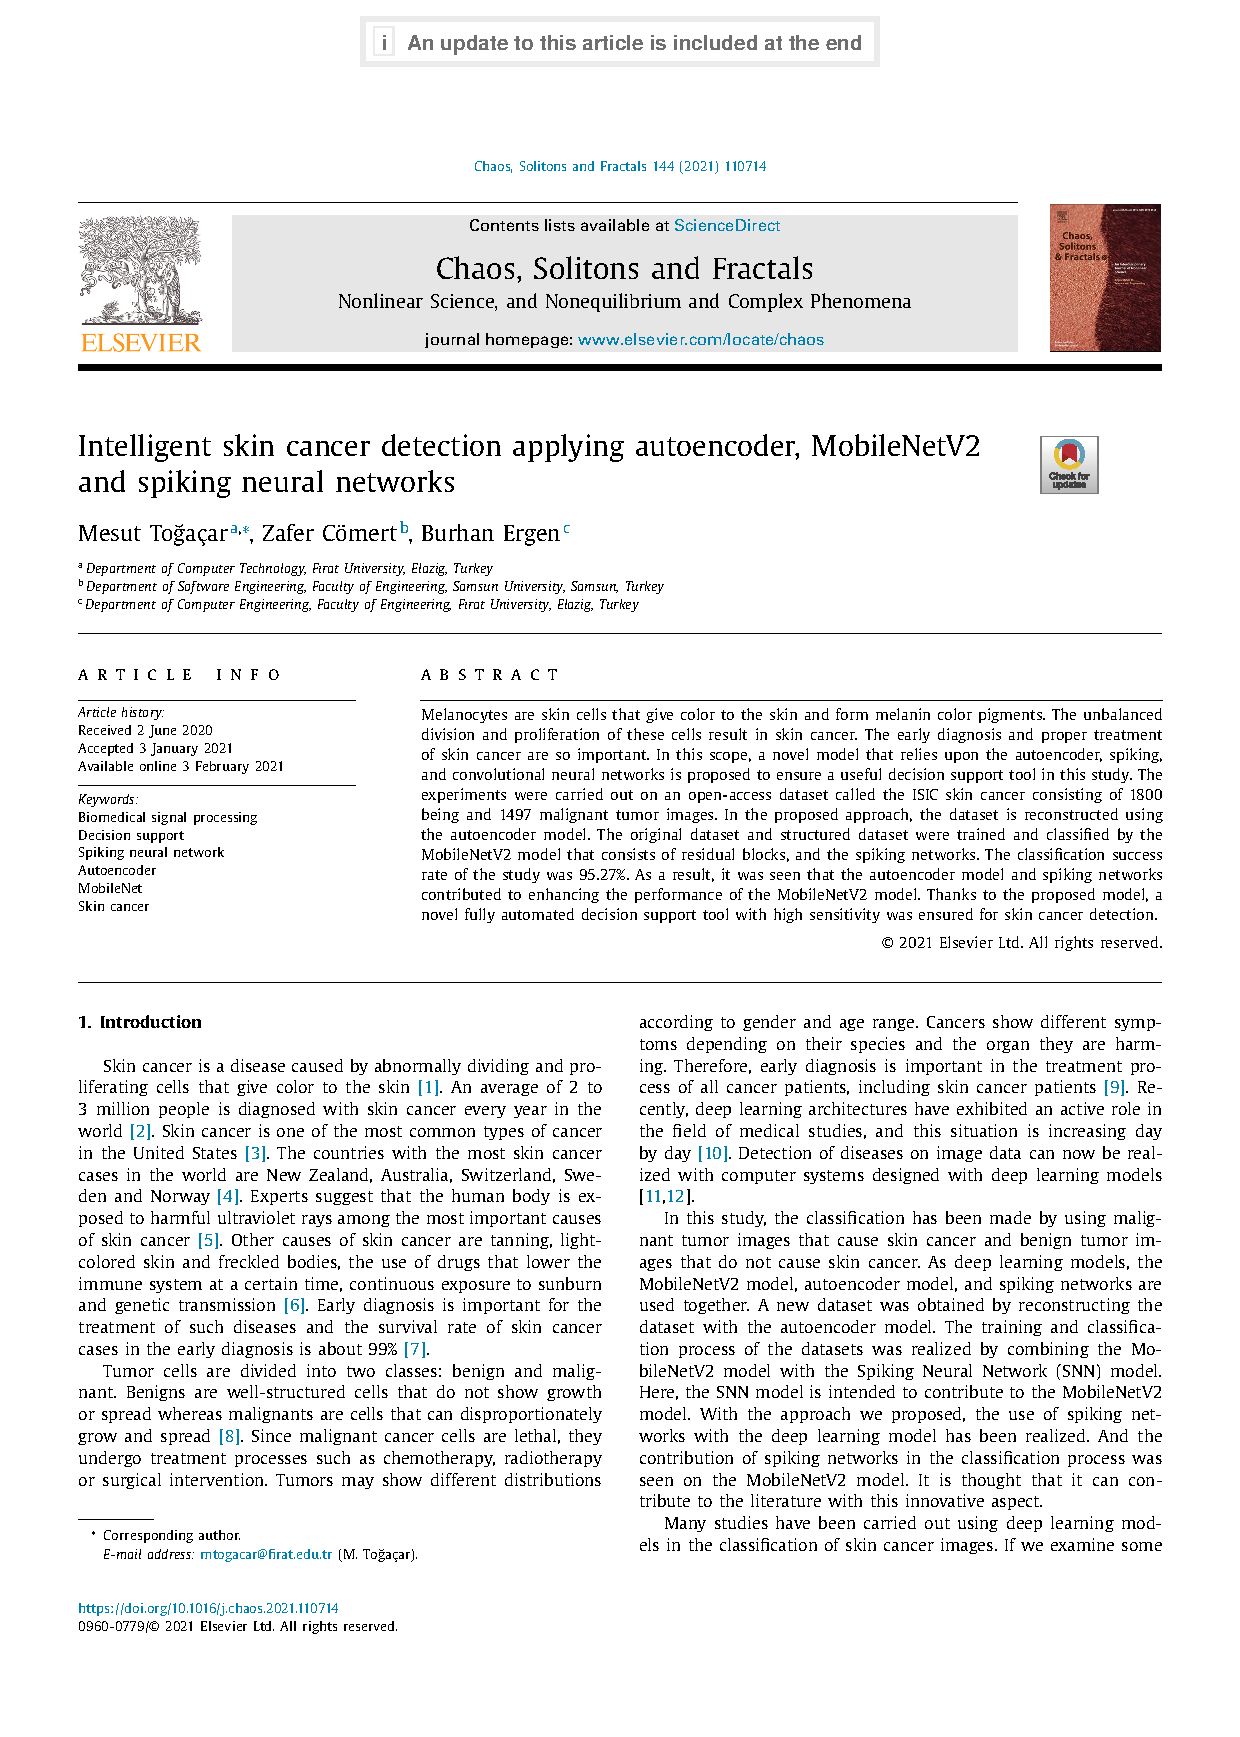
\includegraphics[width=15cm]{./chapter-05-our-contribution/5.png}
    \end{center}
    \caption{This count plot helps to understand the distribution of the data. ~\cite{JULIANA2021}}
    \label{fig:distribution}
    \end{figure}

\section{Pre-processing}
    Before starting the model training process we need to process the dataset, as we learned earlier the dataset consists of around 10015 labeled images for 7 different types of skin lesions, but in our case, we want to get images classified on only two types of skin lesions (Melanoma and Not melanoma). We do this in several steps:

    \begin{description}
        \item[Data cleansing: ] \hfill \\  In this step, we remove unused and damaged data, also repair data that is incorrectly formatted.

        \item[Data separation: ] \hfill \\  After cleansing the data set, we separate the data set into two types of skin lesions by changing the data label for the non-melanoma types to non-melanoma, and we keep the data label for the type of melanoma as it is.

        \item[Data balancing: ] \hfill \\  When reclassifying the data set, we notice that the data set is numerically unbalanced. To solve this problem, we increase the number of images of the melanoma type by rotating, cropping and scaling. As for the non-melanoma type, we reduce the number of images by randomly selecting a specified number of images.

        \item[Image resizing: ] \hfill \\  In this step, we reduce the image size to 75*100 to speed up the training process of the deep learning model. 
        \item[data splitting :] Before the data set becomes usable, we divide it into two parts, the first part is the training set with 80 percent, and the second part is the test set with 20 percent
    \end{description}

        The diagram ~\ref{fig:steps} helps to understand these steps

        \begin{figure}[htbp]
        \begin{center}
        \includegraphics[width=15cm]{./chapter-05-our-contribution/4.png}
        \end{center}
        \caption{Pre-processing}
        \label{fig:steps}
        \end{figure}



\section{Experimental results}
    To judge the performance of the model for the task of predicting skin lesions, we use several evaluation metrics to evaluate our model. This is because the model may perform well using one measurement from one evaluation metric, but may perform poorly using another measurement from another evaluation metric. Using evaluation metrics is critical in ensuring that our model is operating correctly and optimally.

    When the model was trained for 30 epochs, it was observed that the accuracy for both the training and test data started with rather large values and continued to increase slowly from epoch 4 until it reached its peak in epoch 30 (which goes to show that our chosen artchitecture is very good for this task). The test accuracy reached 93 percent and the training accuracy was 97 percent.

    The plot for the accuracy and loss obtained during the training and testing process is shown in Figure ~\ref{fig:acc-loss}

    \begin{figure}[htbp]
    \begin{center}
    \includegraphics[width=15cm]{./chapter-05-our-contribution/1.png}
    \end{center}
    \caption{Accuracy and Loss}
    \label{fig:acc-loss}
    \end{figure}

    The table ~\ref{tab:eval} also includes several other measurements that we used in evaluating our model

    % \setlength{\arrayrulewidth}{0.5mm}
    % \setlength{\tabcolsep}{18pt}
    % \renewcommand{\arraystretch}{1.5}

    \begin{table}[htbp]
    \begin{center}
        \begin{tabular}{|c|c|c|c|c|}
        \hline 
        Classes & Precision & Recall & F1-score & Support \\ 
        \hline 
        Non-melanoma & 0.95 & 0.93 & 0.94 & 1293 \\ 
        \hline 
        Melanoma & 0.93 & 0.95 & 0.94 & 1226 \\ 
        \hline 
        \end{tabular} 
    \end{center}
    \caption{Evaluation Measures}
    \label{tab:eval}
    \end{table}








\chapter{The Diagnosis System}
\section{Conception}
diagrammes
oussama diagram deploiement

\section{Presentation of the Web-based Platform}
hardware
software
app
    auth
    permissions
    interface
    hosting final product in docker containers and charge balancing


\chapter{Conclusion}
Skin cancer is one of the most dangerous and widespread cancers in the world, it can occur to anyone of any age and of any race, just by standing in the sun for too long will increase your chances of getting it. That is why an early diagnosis will save your life. Here where the CAD's (computer aided diagnosis) systems would play an important role by implementing machine learning algorithms that could recognize, detect and classify various skin lesions. Advancements in both machine learning and deep learning have produced a lot of models that reach an accuracy above that of an expert dermatologist, but we can't do without the expertise of specialized doctors.

In this article we have presented a diagnosis system that could facilitate the process of detection and early discovery of melanoma skin cancer, it is web-based, easy to use and accessible to everyone, all you need is internet connection, a laptop or a smartphone, and you are set to go. It can either be used by normal users who think that they might have melanoma, they can check that using the app before actually going to a doctor and do invasive tests (such as biopsy), or it can be used by doctors to facilitate the process of diagnosis and improve patients experience.








\bibliographystyle{unsrt}
\bibliography{bibliography}




\end{document}